%\subsection{One Model vs. Two Models}\label{sec:onevstwo}


\begin{figure}[h!]
\begin{minipage}[b]{0.3\textwidth}
\centering
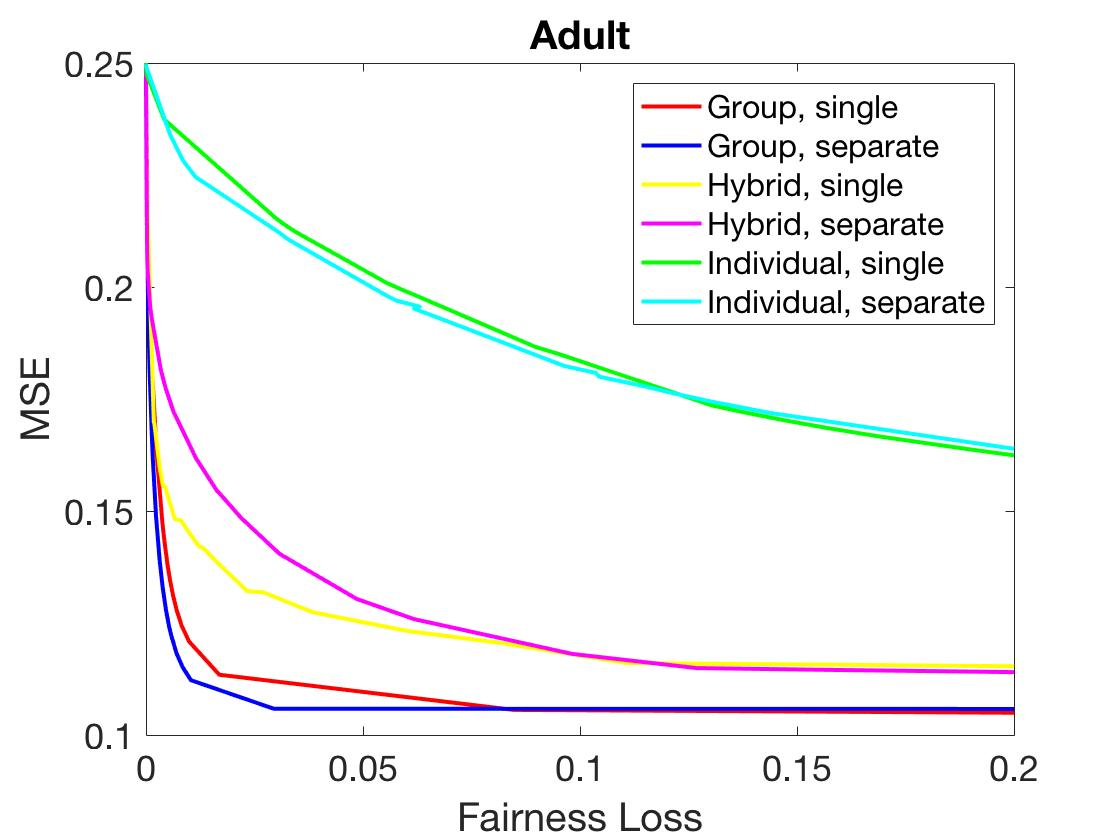
\includegraphics[width=5cm]{./figures/twoversusone-adult.jpg}
%\caption{}
\end{minipage}
\begin{minipage}[b]{0.3\textwidth}
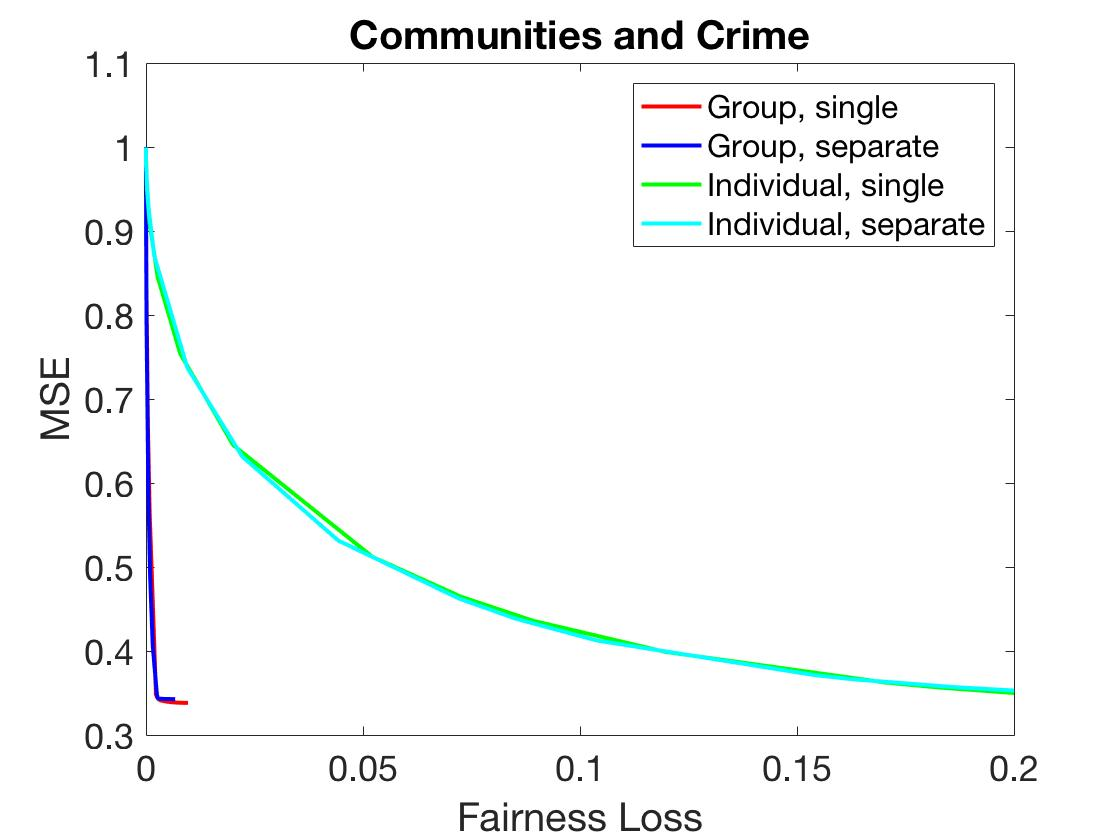
\includegraphics[width=5cm]{./figures/twoversusone-communities.jpg}
%\caption{}
\end{minipage}
\begin{minipage}[b]{0.3\textwidth}
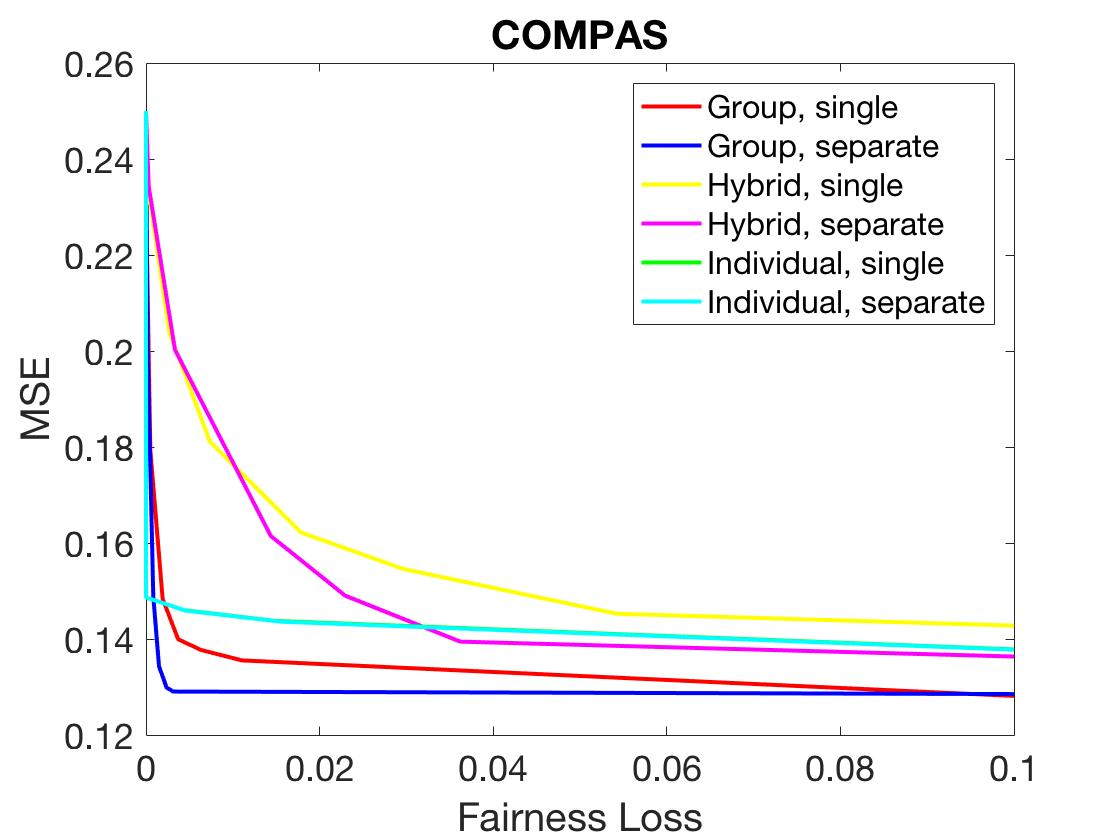
\includegraphics[width=5cm]{./figures/twoversusone-compas.jpg}
%\caption{}
\end{minipage}\\
\begin{minipage}[b]{0.3\textwidth}
\centering
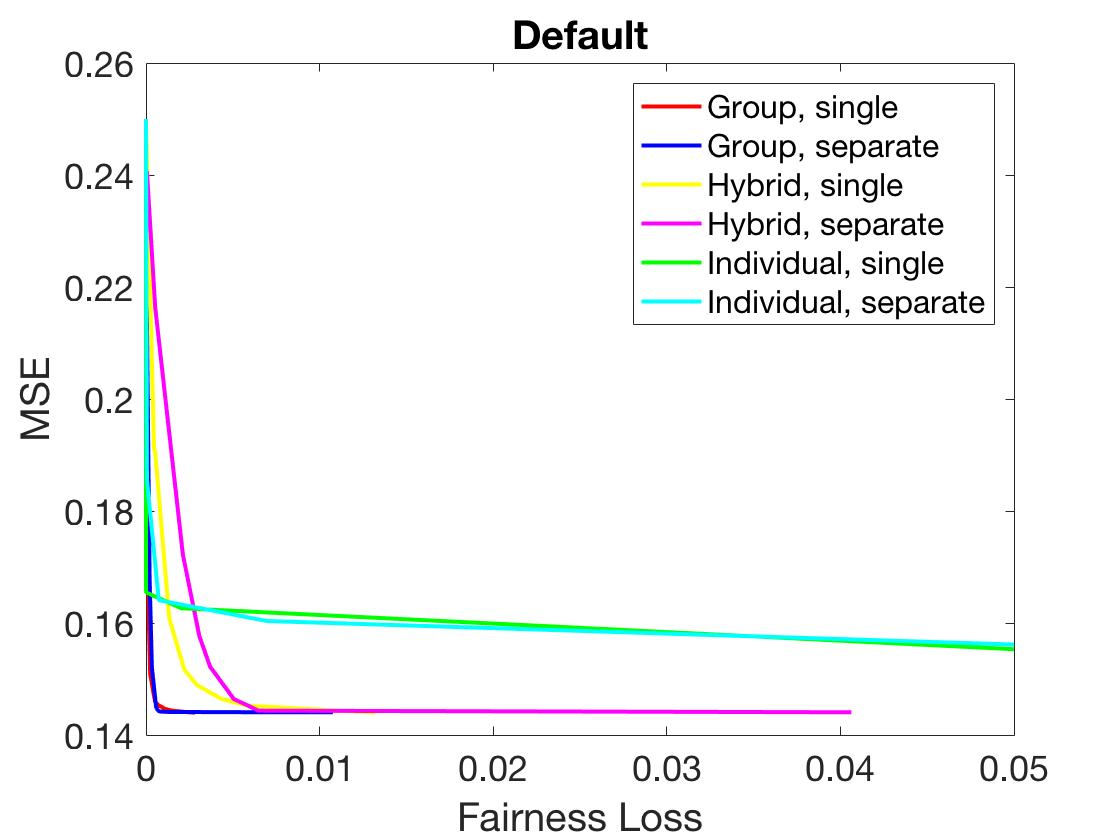
\includegraphics[width=5cm]{./figures/twoversusone-default.jpg}
%\caption{}
\end{minipage}
\begin{minipage}[b]{0.3\textwidth}
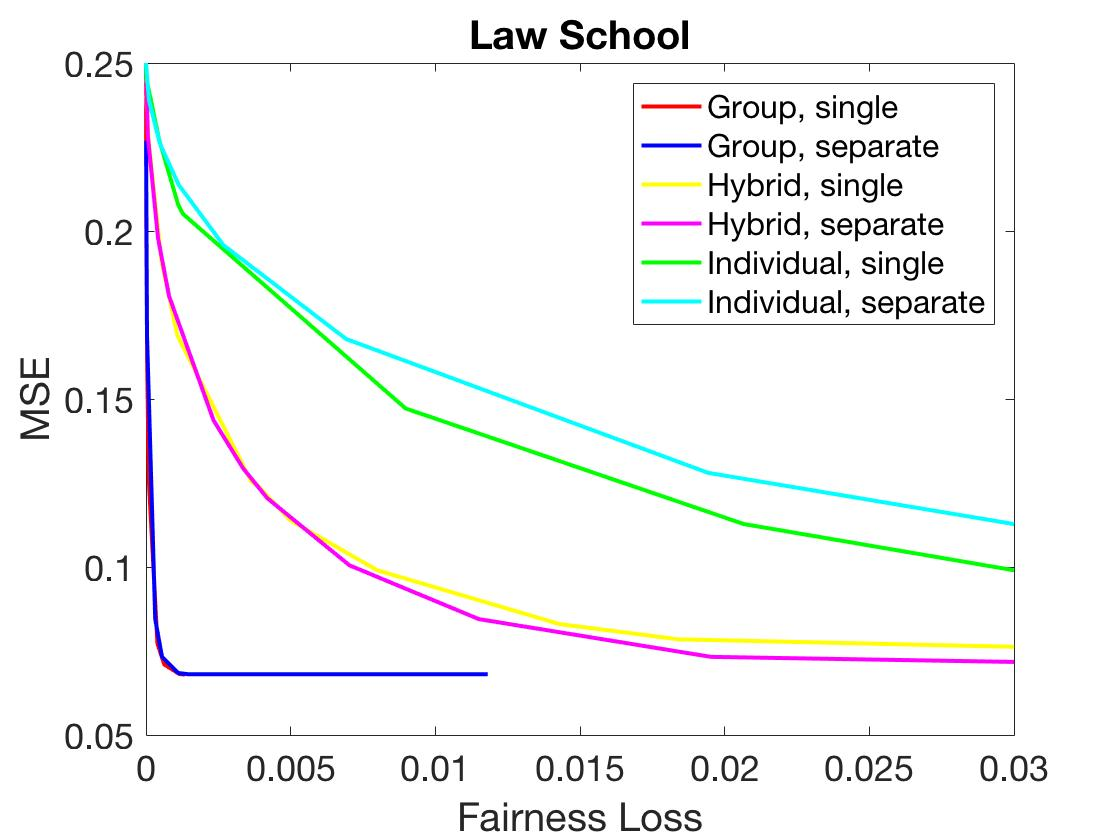
\includegraphics[width=5cm]{./figures/twoversusone-law.jpg}
%\caption{}
\end{minipage}
\begin{minipage}[b]{0.3\textwidth}
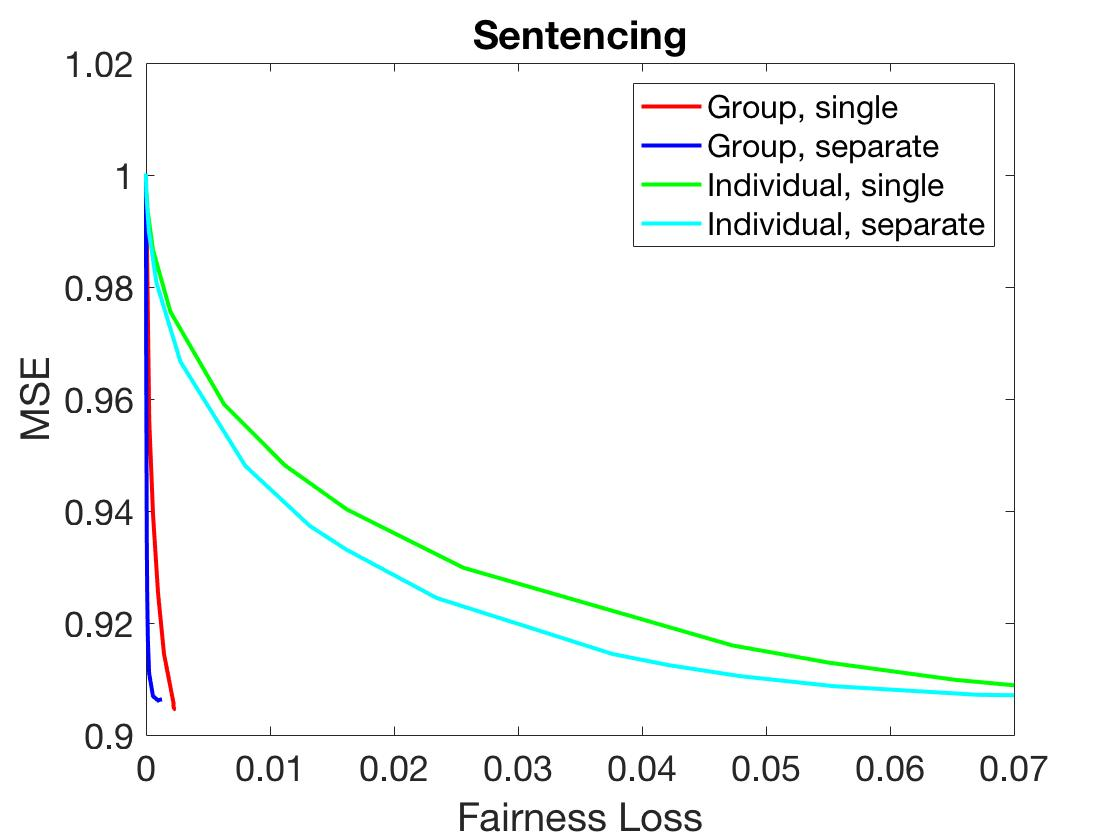
\includegraphics[width=5cm]{./figures/twoversusone-philadelphia.jpg}
%\caption{}
\end{minipage}
\caption{Efficient frontiers of accuracy vs. fairness for each dataset. For datasets with binary-valued
targets (logistic regression), we consider three fairness notions (group, individual and hybrid), and
for each examine building a single model or separate models for each group, yielding a total of six curves.
For real-valued targets
(linear regression), we consider two fairness notions (group and individual), and again single or
separate models, yielding a total of four curves.
\label{fig:pareto}}
\end{figure}

